\documentclass[a4paper]{oblivoir}
\usepackage{amsmath,amssymb,kotex,kswrapfig,mdframed,paralist,graphicx}
\usepackage{fapapersize}
\usefapapersize{210mm,297mm,20mm,*,20mm,*}

\usepackage{tabto,pifont}
\TabPositions{0.2\textwidth,0.4\textwidth,0.6\textwidth,0.8\textwidth}
\newcommand\tabb[5]{\par\noindent
\ding{172}\:{\ensuremath{#1}}
\tab\ding{173}\:\:{\ensuremath{#2}}
\tab\ding{174}\:\:{\ensuremath{#3}}
\tab\ding{175}\:\:{\ensuremath{#4}}
\tab\ding{176}\:\:{\ensuremath{#5}}}

\usepackage{tabu}

\pagestyle{empty}
%%% Counters
\newcounter{num}

%%% Commands
\newcommand\defi[1]
{\bigskip\par\noindent\stepcounter{num} \textbf{정의 \thenum) #1}\par\noindent}
\newcommand\theo[1]
{\bigskip\par\noindent\stepcounter{num} \textbf{정리 \thenum) #1}\par\noindent}
\newcommand\exam[1]
{\bigskip\par\noindent\stepcounter{num} \textbf{예시 \thenum) #1}\par\noindent}
\newcommand\prob[1]
{\bigskip\par\noindent\stepcounter{num} \textbf{문제 \thenum) #1}\par\noindent}

\newcommand\pb[1]{\ensuremath{\fbox{\phantom{#1}}}}

\newcommand\an[1]{\bigskip\par\noindent\textbf{문제 #1)}\par\noindent}

\newcommand\ba{\ensuremath{\:|\:}}

\newcommand\vs[1]{\vspace{20pt}}

%%% Meta Commands
\let\oldsection\section
\renewcommand\section{\clearpage\oldsection}

\let\emph\textsf

\begin{document}
\begin{center}
\LARGE민형, 미니테스트 03
\end{center}
\begin{flushright}
날짜 : 2017년 \(\pb3\)월 \(\pb{10}\)일 \(\pb{월}\)요일
,\qquad
제한시간 : \pb{17년}분
,\qquad
점수 : \pb{20} / \pb{20}
\end{flushright}

%미4유3
\prob{}
다음을 계산하시오.
\begin{enumerate}[(1)]
\item
\(\displaystyle\lim_{x\to0}\frac{\sin 3x}{2x}\)
\item
\(\displaystyle\lim_{x\to0+}\frac{3x}{\tan x}\)
\item
\(\displaystyle\lim_{x\to0}\frac{1-\cos x}{x^2}\)
\item
\(\displaystyle\lim_{x\to0}\frac{\sin 2x}{x+\sin3x}\)
\end{enumerate}
\vs

%미4고2
\prob{}
함수 \(f(x)=\cos x-3x\)에 대하여 \(\displaystyle\lim_{x\to0}\frac{f(\tan4x)-f(\sin6x)}{x}\)의 값은?
\tabb68{10}{12}{14}
\vs

%미4수3
\prob{}
그림과 같이 반지름의 길이가 \(r\)이고 중심각의 크기가 \(\theta\)인 부채꼴 \(OAB\)애 내접하는 원을 \(C\)라고 하자.
호 \(AB\)의 길이를 \(l\), 원 \(C\)의 둘레의 길이를 \(m\)이라고 할 때, \(\displaystyle\lim_{\theta\to0+}\frac ml\)의 값은?
\begin{figure*}[h!]
\centering
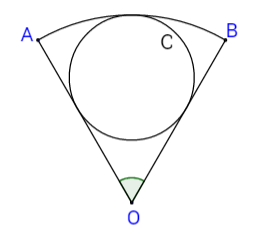
\includegraphics{inscribed_circle}
\end{figure*}
\tabb1{\frac12}{\frac\pi4}{\frac\pi2}\pi
\vs

%
\prob{}
다음을 적분하시오.
\begin{enumerate}[(1)]
\item
\(\displaystyle\int_0^\pi\sin x\,dx\)
\item
\(\displaystyle\int_0^\pi\sin^2x\,dx\)
\item
\(\displaystyle\int_0^\pi\sin^3x\,dx\)
\item
\(\displaystyle\int_0^\pi\sqrt{2-2\cos x}\,dx\)
\end{enumerate}

\clearpage
\begin{tabu}{|c|c|c|c|c|c|c|c|c|c|}
\hline
문제1, (1)&(2)&(3)&($)&문제2&문제3&문제4, (1)&(2)&(3)&(4)
\\\hline
\(\frac32\)&\(3\)&\(\frac12\)&\(\frac12\)&\ding{172}&\ding{176}&\(2\)&\(\frac\pi2\)&\(\frac43\)&\(4\)
\\\hline
\end{tabu}

\end{document}